\documentclass[xcolor=dvipsnames]{beamer} 
\usecolortheme[named=Brown]{structure} 
\usetheme[height=7mm]{Rochester} 

\setbeamertemplate{items}[default] 
\setbeamertemplate{itemize subitem}[circle] % if you wnat a circle

\usepackage[spanish]{babel}
\usepackage[utf8]{inputenc}

\usepackage{graphicx}

\usepackage{color}
\usepackage{listings}
\lstset{ %
language=Prolog,            % choose the language of the code
breaklines=true,            % sets automatic line breaking
frame=single,               % Add a frame to listings.
basicstyle=\footnotesize,   % Font size.
}

% items enclosed in square brackets are optional; explanation below
\title{El lenguaje de programación Prolog}
\subtitle{Presentación para la materia Teoría del Lenguaje}
\author{
Axel Straminsky \\
Demian Ferrerio \\
Martín Paulucci
}
\institute[UMBC]{
  Facultad de Ingeniería\\
  Universidad de Buenos Aires \\
}
\date{9 de Mayo, 2011}

\newtheorem{codigo}{Código}

\begin{document}

%--- the titlepage frame -------------------------%
\begin{frame}[plain]
  \titlepage
\end{frame}

\begin{frame}{Visión General}

\begin{itemize}
\item Es el lenguaje más famoso del Paradigma Lógico
\item Un programa Prolog consiste en un conjunto de sentencias, que pueden ser hechos o reglas.
\item Es conversacional. La interacción con el programa consiste en hacerle preguntas al sistema.
\item Usado en Inteligencia Artificial y procesamiento de Lenguajes Naturales.
\end{itemize}

\end{frame}

\begin{frame}{Historia}

\begin{itemize}
\item Su nombre proviene de la abreviación \textit{PROgramming in LOGic}.
\item Fue ideado a principios de los '70 por Colmerauer y Roussel.
\item Nació de un proyecto que no tenía como objetivo la implementación de un lenguaje de programación, sino el procesamiento de lenguajes naturales.
\item Inicialmente interpretado,  hasta que en 1983 se desarrollo un compilador capaz de traducir Prolog a un conjunto de instrucciones de una máquina abstracta denominada Warren Abstract Machine (WAM), y desde entonces Prolog es semi-interpretado.
\end{itemize}

\end{frame}

\begin{frame}{Declaratividad}
 
\begin{itemize}
 \item Describe la \emph{lógica} del programa sin explicitar el flujo de ejecución.
 \begin{itemize}
  \item Lo opuesto a la programación imperativa.
 \end{itemize}
 \item Permite abstraerse del “cómo” y concentrarse en el “qué” a la hora de escribir programas.
 \item El paradigma Lógico, al igual que el Funcional, provienen del paradigma Declarativo.
 \item Programar de esta manera tiende a reducir los errores causados por ``efectos colaterales'' (side effects).
 \item Ideal para implementar Computación Paralela
\end{itemize}

\end{frame}

\begin{frame}{Paradigma Lógico}

\begin{itemize}
\item Puramente declarativo, es decir, no tiene estructuras de control.
\item La lógica matemática es la manera más sencilla de expresar formalmente problemas complejos para el intelecto humano.
\item Las resonsabilidades para la ejecución de una tarea están divididas entre el programador, que debe asegurar que el modelo sea lógicamente coherente, y la máquina, que debe resolver el problema de manera eficiente.


Los lenguajes lógicos usan sobre todo para las siguientes aplicaciones:

\begin{columns}
  \begin{column}{0.45\textwidth}
  \begin{itemize}
    \item Inteligencia Artificial
    \item Demostración automática de Teoremas
  \end{itemize}
  \end{column}

  \begin{column}{0.45\textwidth}
  \begin{itemize}
    \item Sistemas expertos
    \item Reconocimiento de Lenguaje Natural
  \end{itemize}
  \end{column}
\end{columns}

\end{itemize}

\end{frame}

\begin{frame}{Implementaciones de Prolog}

    Algunas implementaciones de Prolog son:

    \begin{itemize}
    \item SWI-Prolog : soporta Mulithreating.
    \item Mercury : Mezcla de Programación Lógica y Funcional.
    \item Fprolog: Añade lógica difusa.
    \item Prolog+ : Añade Clases y jerarquías de Clases.
    \item LogTalk: Añade \textit{POO}.
    \item $\lambda$prolog: Soporta Polimorfismo y Programación de Alto Nivel.
    \end{itemize}

\end{frame}

\begin{frame}[fragile]{Programación en Prolog: Hechos y Términos simples}

    \begin{itemize}
        \item Un programa Prolog puro está compuesto únciamente de un conjunto finito de \textit{Clausulas de Horn}. Hay dos tipos de clausulas: \textit{hechos} y \textit{reglas}.
        \item Un \textit{hecho} define una verdad del programa. Por ejemplo:
        \begin{lstlisting}
        varon(pedro).
        \end{lstlisting}
        puede leerse ``Pedro es un varón''.
        \item ``Sólo un tipo de dato'': el término
        \item Existen términos atómicos (e.g. \verb|pedro|, \verb|x|, \verb|'un atomo'|)
        \item Numéricos (e.g. \verb|6|, \verb|-15|).
        \item Compuestos
        \begin{itemize}
            \item Por ejemplo \verb|gusta(martin, jazz)| \\
            Donde \verb|gusta| es un \textit{functor} (o predicado), que se caracteriza por un nombre y aridad; y se denota \verb|gusta/2|. \\
            Y \verb|martin| y \verb|jazz| son átomos, que tambien pueden verse como functores de aridad cero.
        \end{itemize} 
    \end{itemize} 

\end{frame}

\begin{frame}[fragile]{Programación en Prolog: Variables y Reglas}
    \begin{itemize}
        \item Una lista es un caso especial de término compuesto \\
        e.g. \verb|[1, 2, 3, 5]|
        \item Una \textit{variable} representa un valor no especificado.
        \item Sintaxis: los átomos y predicados con minúscula y las variables con mayúscula.
        \item Una \textit{regla} define una relación del tipo: 
        \[
        (p \wedge q \wedge \cdots \wedge t) \Rightarrow u
        \]
        \item En Prolog, se escribe primero el consecuente, y después el o los antecedentes. Por ejemplo:
        \begin{lstlisting}
hija(A, B) :- mujer(A), madre(B, A).
        \end{lstlisting}
    \end{itemize}
\end{frame}

\begin{frame}[fragile]{Programación en Prolog: Queries}
    Las queries son la forma de obtener información del programa.
    \begin{itemize}
        \item Si se especifican todos los parámetros de una consulta con constantes, el intérprete informa si el predicado se cumple o no.
        \begin{lstlisting}
?- factorial(5, 120).
true .
        \end{lstlisting} 
        \item Si alguno de los términos de la consulta es una variable, se informa qué valores debe tomar la variable para cumplir ese predicado.
        \begin{lstlisting}
?- hermano(zeus, Quien).
Quien = hades ;
Quien = poseidon ;
false.
        \end{lstlisting} 
    \end{itemize}
\end{frame}

\begin{frame}[fragile]{Programación en Prolog: Reglas recursivas}
    \begin{itemize}
        \item Ejemplo de regla recursiva:
        \begin{lstlisting}
ancestro(A, B) :- padre(A, B).
ancestro(A, B) :- padre(A, X), ancestro(X, B).
        \end{lstlisting} 
        \begin{itemize}
            \item Las condiciones de corte se especifican como hechos.
        \end{itemize}
        \item Ver ejemplo \verb|ancestro.pl|
    \end{itemize}
\end{frame}

\begin{frame}[fragile]{Ejemplo: Factorial}
 
\begin{itemize}
 \item En Prolog no existen instrucciones de control, y su ejecución se basa en 2 conceptos: \textit{unificación} y \textit{backtracking}. 
 \item La unificación produce una ligadura entre 2 términos lógicos que están relacionados mediante una igualdad.
 \item Veamos un ejemplo:
\lstinputlisting{../src/factorial.pl}
\begin{itemize}
 \item El flujo de control se genera utilizando recursividad.
 \item Se usa como función de corte a los hechos. 
\end{itemize}
\end{itemize}

\end{frame}
 
\begin{frame}[fragile]{Backtracking}
 
    Ejemplo de seguimiento.
    \begin{lstlisting}
?- factorial(3, 6).
true .
    \end{lstlisting}
    % http://www.lucidchart.com/documents/demo/4dc83d9c-7014-49fa-85c8-2b3a0a7a6b76
    \begin{figure}[H]
		\centering
		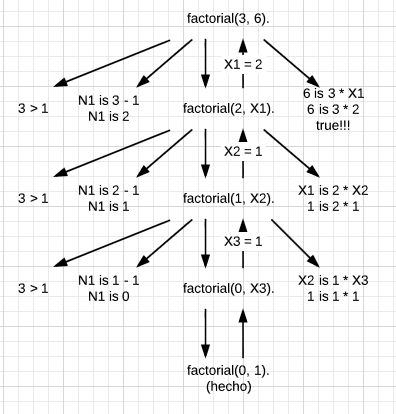
\includegraphics[height=175pt]{factorial.png}
	\end{figure}

\end{frame}

\begin{frame}[fragile]{Ejemplos interesantes}
Ver ejemplos \verb|cambio.pl| y \verb|n_reinas.pl|.
\end{frame}

\begin{frame}[fragile]{Desventajas de Prolog}
    \begin{itemize}
        \item Prolog no es un lenguaje de proposito general.
        \item No tiene un sistema de módulos, lo cual hace que sea poco escalable.
        \item No hay un estandard bien definido
        \begin{itemize}
            \item Incompatibilidades entre distintas implementaciones.
        \end{itemize}
        \item Baja performance en comparación con otros lenguajes.
        \begin{itemize}
            \item Poco apropiado para programas computacionalmente complejos.
        \end{itemize}
    \end{itemize}
\end{frame}

\begin{frame}[fragile]{Fin}
    Preguntas \\
    \pause
    Muchas gracias!
\end{frame}


\end{document}
